% -- ACM --
% \documentclass[sigconf,anonymous,review=true,natbib=false]{acm-template/acmart}
% \documentclass[sigconf,anonymous,review]{acm-template/acmart}

% -- IEEE --
\documentclass[conference]{ieee-template/IEEEtran}
\IEEEoverridecommandlockouts

% -- we use biblatex instead of bibtex --
\usepackage[
  % datamodel=acm-template/acmdatamodel,  % ACM-specific
  style=numeric-comp,
  backend=biber,
  sorting=none % produces compressed ranges
]{biblatex}

% bib customizations
\DeclareSourcemap{
  \maps[datatype=bibtex]{
    \map{ % suppress "(visited on ...)"
      \step[fieldset=urldate, null]
    }
  }
}

\usepackage{listings} % -- for code blocks --
\usepackage{xcolor}
\usepackage{algorithm}
\usepackage{algpseudocodex}
\usepackage{inconsolata} % change texttt font from ugly IEEE defaults
\usepackage{sourcesanspro} % change textsf font from ugly IEEE defaults
\usepackage{tabularx}
\usepackage{float} % for [H] non-floating placement
% \usepackage{balance} % balance columns on last page
% \usepackage{flushend} % balance columns on last page
\usepackage{pbalance} % balance columns on last page, works

% -- cleveref + config --
\usepackage{amsmath} % for \text{}, must be loaded before cleveref
\usepackage{cleveref}
\crefname{figure}{fig.}{figs.}
\Crefname{figure}{Fig.}{Figs.}

% -- caption spacing ---
\usepackage[skip=4pt, font={small,bf}]{caption} % skip=4pt above caption
\setlength{\textfloatsep}{6pt plus 2pt minus 2pt} % skip = 6 +- 2pt below caption
\setlength{\floatsep}{6pt plus 2pt minus 2pt} % skip = 6 +- 2pt below caption

\usepackage{subcaption}
\usepackage{enumitem} % for wide lists
\usepackage{booktabs} % for \toprule, \midrule, \bottomrule
\usepackage{multirow} % for \multirow in tables
\usepackage[switch]{lineno} % draft line numbers; switch puts numbers on outer margins


% -- local resources --
\graphicspath{{./data/figs/}{./data/tikz-figs-new/pdf/}{./data/thesis-figs/}}
\addbibresource{bib/NetSketch-Mon.bib}
\addbibresource{bib/claude.bib}
\addbibresource{bib/General-Thesis.bib}

% -- Macros --
% -- para headings --
\newcommand{\parahead}[1]{%
  \vspace{0.2em}\noindent\emph{#1.}\space
}

\newcommand{\pplushead}[1]{%
  \vspace{0.25em plus 0.1em minus 0.1em}\noindent\emph{#1.}\space
}

% -- TODO macro --
\newcommand{\todo}[1]{%
  \textcolor{red}{TODO: #1}%
}

% -- Citation key macros --
\newcommand{\citeJainAmr}{Jain2025:AMR}
% \newcommand{\citeJainAmr}{anon:paper}
% arXiv, seems to have been accepted as Cui2026:Flare at NSDI 2026, but full text not available
\newcommand{\citeCuiXputimer}{Cui2025:XPUTimer}

% -- Citation group macros --
\newcommand{\citeGroupML}{Yao2025:Holmes,Wu2025:GREYHOUND,\citeCuiXputimer,Guan2025:PerfTracker,Deng2025:Mycroft,Chen2025:Reveal,Dong2025:Aegis,Deng2025:Minder,Jiang2025:TrainCheck}
\newcommand{\citeGroupVarHpc}{Petri2003:Missing,Acun2016:Variation,Gunaw2018:FailSlow,Bhate2020:PerfVar}
\newcommand{\citeGroupVarAmr}{VanS2009:AMR,\citeJainAmr}
\newcommand{\citeGroupVarRdma}{Kong2022:Collie,Gangi2024:RDMA}
\newcommand{\citeGroupVarMisc}{You2024:GVARP,Lu2023:PERSEUS,Yildi2016:IONoise}
% -- Unused: tool/solution papers for variability --
\newcommand{\citeGroupVarSolns}{Kocol2018:Varbench,Xuan2025:STAD,Acun2016:Mitigating}

% -- Tilde macro --
\newcommand{\mytilde}{{\raise.17ex\hbox{$\scriptstyle\sim$}}}

% -- Tool name macros --
\newcommand{\scorep}{Score-P}
\newcommand{\dftracer}{DFTracer}
\newcommand{\qlogic}{QLogic}
\newcommand{\mpiw}{\texttt{MPI\_Wait}}

% -- Protocol macro --
\newcommand{\twopc}{\textsf{TS2PC}}

% -- TBON tier macros --
\newcommand{\tierctl}{\textsf{CTL}}
\newcommand{\tieragg}{\textsf{AGG}}
\newcommand{\tiermpi}{\textsf{MPI}}

% -- Flow marker (matches agentic_timeline.py) --
\definecolor{flowblue}{HTML}{b3cde3}
\newcommand{\flowmark}[1]{%
  \tikz[baseline=(char.base)]{
    \node[fill=flowblue,text=black,circle,inner sep=1pt,font=\small\bfseries,draw=black,line width=0.3pt] (char) {#1};
  }%
}

% ! TeX root = ../main.tex

% Background: Volatile function tail latency example
\newcommand{\figBgVolatile}{%
  \begin{figure}[t]
    \centering
    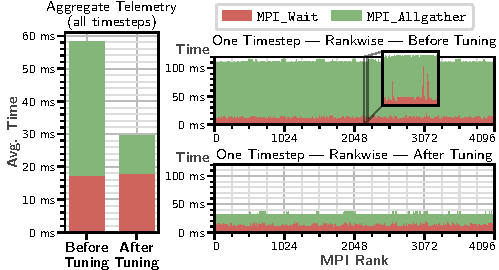
\includegraphics[width=\columnwidth]{lesson_volfunc_zoom.pdf}
    % \caption{Simplified view of telemetry from a real BSP app with a volatile function followed by a global collective.
    %   Tail latency in the volatile function gets misattributed as elevated collective time in aggregate
    %   telemetry (left), but not in fine-grained telemetry (right).
    % }
    % \caption{Telemetry from an AMR code where a volatile \mpiw{} precedes \texttt{MPI\_Allgather}.
    %   Aggregate telemetry (left) misattributes straggler-induced \mpiw{} as elevated collective cost.
    %   Fine-grained telemetry (right) makes the cause obvious but requires joining all ranks' telemetry.
    % }
    \caption{Reproduced performance pathology from an AMR code~\cite{\citeJainAmr}.
      A volatile \mpiw{} preceding \texttt{MPI\_Allgather} is misattributed as elevated collective cost
      in aggregate telemetry (left).
      Rank-level telemetry for a single timestep (right) reveals the true cause but requires joining all
      ranks' data.
    }
    \label{fig:orca:bg-volatile}
  \end{figure}%
}

% Design: ORCA Architecture
\newcommand{\figDesignArch}{%
  \begin{figure}[t]
    \centering
    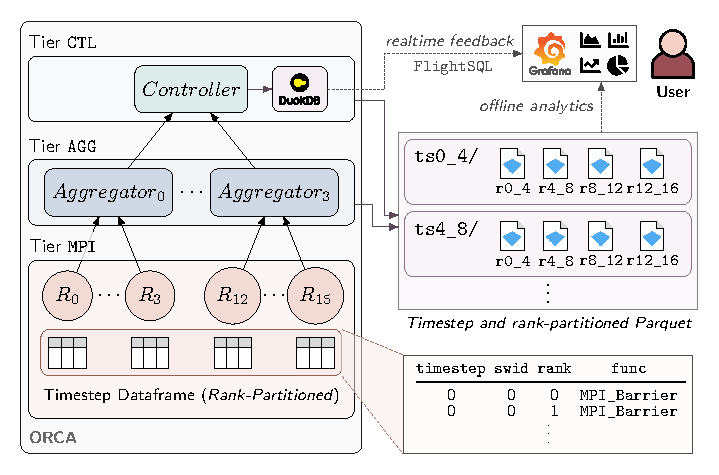
\includegraphics[width=0.48\textwidth, trim=0.2cm 0cm 0.2cm 0cm, clip]{thesis-orca-arch.pdf}
    % \caption{ORCA architecture.
    %   A three-tier TBON with application ranks (\tiermpi{}) at the leaves, aggregator nodes (\tieragg{})
    %   at intermediate levels, and a controller (\tierctl{}) at the root.
    %   Data flows upward as columnar Arrow streams, transformed en-route by OrcaFlow operators, and
    %   persisted via Parquet or DuckDB sinks.
    % }
    \caption{ORCA architecture.
      A three-tier TBON with application ranks (\tiermpi{}) at the leaves, intermediate aggregators
      (\tieragg{}), and a controller (\tierctl{}) at the root.
      Telemetry originates as columnar timestep dataframes, is transformed by SQL plan operators at each
      tier, and persisted via DuckDB and Parquet sinks --- enabling workflows from real-time feedback via
      lightweight metrics to zero-ETL post-hoc analytics.
    }
    \label{fig:orca:des-arch}
  \end{figure}%
}

% Design: ORCA Flow Plan
\newcommand{\figDesignPlan}{%
  \begin{figure}[t]
    \centering
    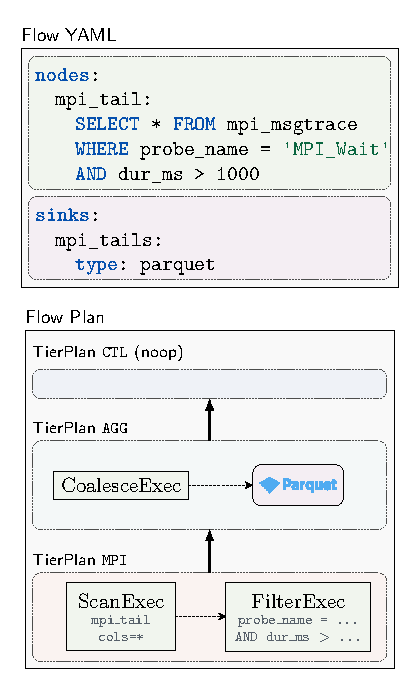
\includegraphics[width=0.24\textwidth, trim=0.35cm 0cm 0.2cm 0.4cm, clip]{plan.pdf}%
    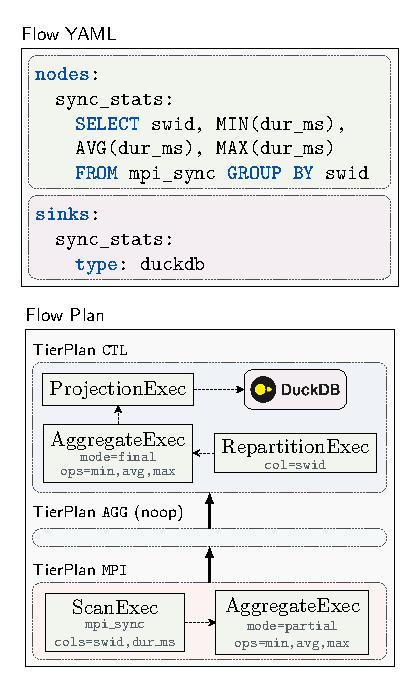
\includegraphics[width=0.24\textwidth, trim=0.3cm 0cm 0.3cm 0.4cm, clip]{plan2.pdf}
    % \caption{OrcaFlow compilation. (Left) An OrcaFlow definition specifying SQL transforms over
    %   telemetry streams. (Right) The compiled tier plans showing operator placement across
    %   \tiermpi{}, \tieragg{}, and \tierctl{}, with filters pushed to leaves and aggregation
    %   at higher tiers.}
    \caption{OrcaFlow compilation showing flows and their compiled tier plans.
      Flows chain SQL transforms over telemetry streams en route to configurable sinks.
      Both operators and sinks are placed automatically.
      (Left) A selective filter pushed to \tiermpi{}, discarding most data at source.
      (Right) Aggregations also reduce data volume --- pushed-down partial aggregations emit fixed-size intermediates regardless of input volume.
    }
    \label{fig:orca:des-plan}
  \end{figure}%
}

% Design: \twopc{} Protocol
\newcommand{\figDesignTwopc}{%
  \begin{figure}[t]
    \centering
    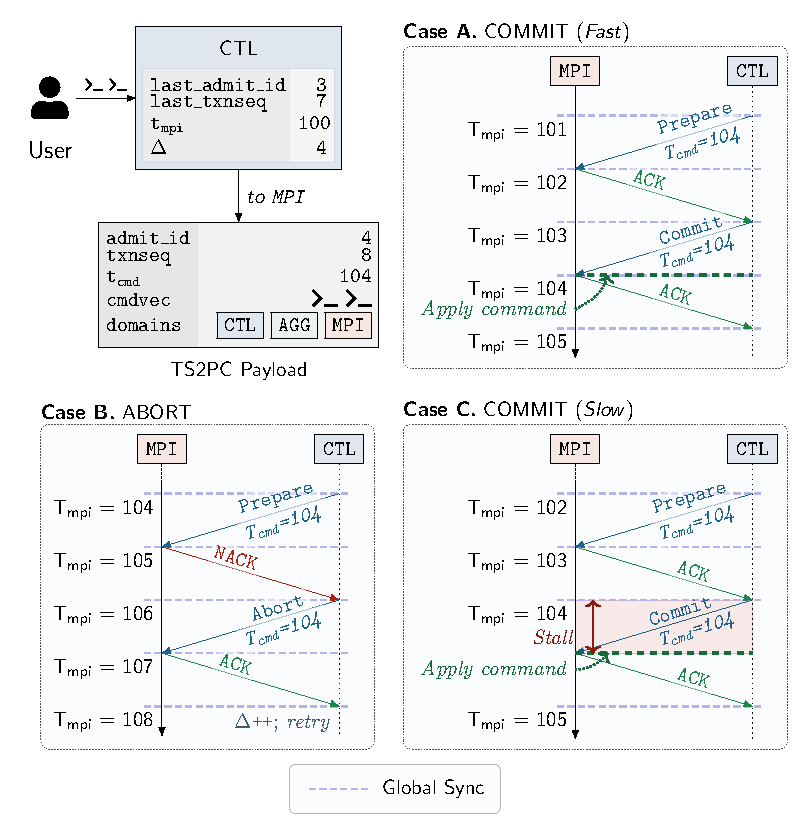
\includegraphics[width=0.48\textwidth, trim=0.2cm 0cm 0.2cm 0cm, clip]{ts2pc_paper.pdf}
    \caption{Timestep-linked two-phase commit (\twopc{}).
      Commands are proposed for a future timestep $T_{cmd} = T_{mpi} + \Delta$.
      (A) Normal case: ranks agree and apply the command before executing $T_{cmd}$.
      (B) Abort: ranks have passed $T_{cmd}$ and vote to abort, command is retried with a
      larger $\Delta$. (C) Stall: ranks have prepared but not received commit/abort.
      Execution blocks until resolution to preserve correctness.
    }
    \label{fig:orca:des-twopc}
  \end{figure}%
}

% Eval: Runtime, trace size, query suite (3 subfigures)
\newcommand{\figEvalBannerAll}{%
  \begin{figure*}[t]
    \begin{subfigure}[t]{\textwidth}
      \centering
      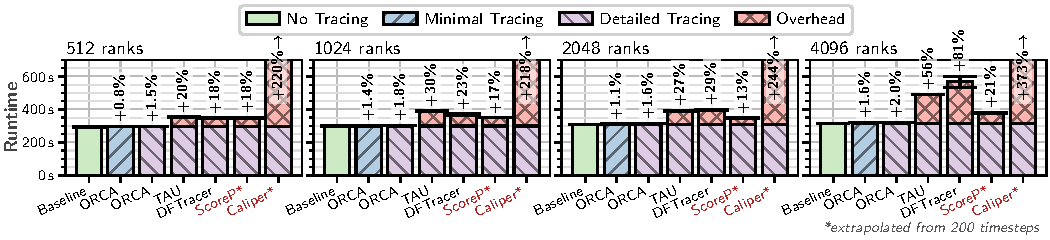
\includegraphics{amr_tracer_runtimes.pdf}
      \caption{Runtime overhead.}
      \label{fig:orca:eval-banner-runtime}
    \end{subfigure}
    \begin{subfigure}[t]{0.49\textwidth}
      \centering
      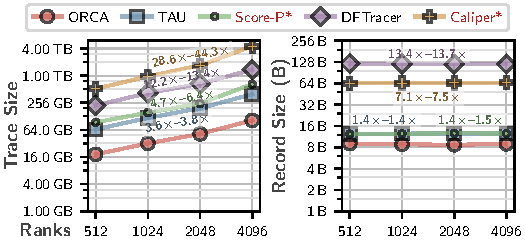
\includegraphics[width=\textwidth]{amr_tracesizes_line.pdf}
      \caption{Storage efficiency.}
      \label{fig:orca:eval-banner-size}
    \end{subfigure}
    \hfill
    \begin{subfigure}[t]{0.49\textwidth}
      \centering
      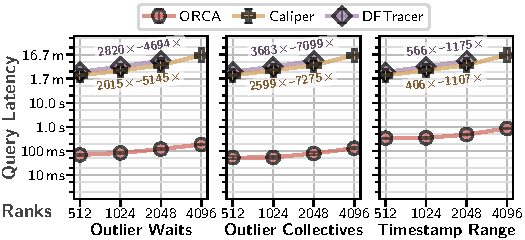
\includegraphics[width=\textwidth]{query_suite_abs.pdf}
      \caption{Query performance.}
      \label{fig:orca:eval-banner-query}
    \end{subfigure}
    \caption{ORCA substrate evaluation at 512--4096 ranks. (Top) Runtime overhead: ORCA maintains
      0.8--2\% while traditional tracers degrade to 56--81\% at scale. (Bottom-left) Storage:
      Parquet is 2--20$\times$ smaller than alternatives. (Bottom-right) Query latency: ORCA is
      3--4 orders of magnitude faster due to columnar format and partition pruning.}
    \label{fig:orca:eval-banner}
  \end{figure*}%
}

% Eval: Runtime overhead, two-column
\newcommand{\figEvalOverhead}{%
  \begin{figure*}[t]
    \centering
    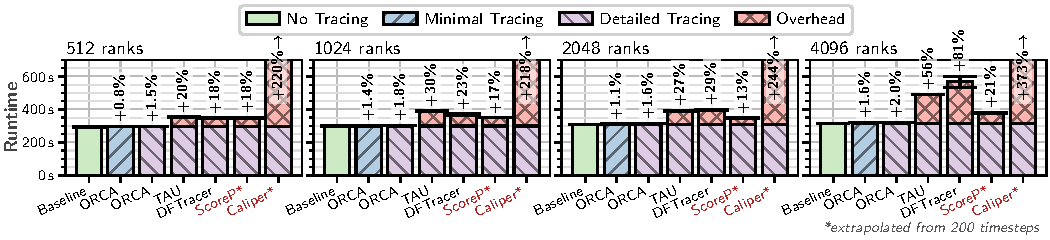
\includegraphics[width=\textwidth]{amr_tracer_runtimes.pdf}
    % \caption{Runtime overhead comparison at 512--4096 ranks.
    %   ORCA maintains 0.8--2\% overhead across all scales and profiles, while traditional tracers degrade
    %   from 18--20\% at 512 ranks to 56--81\% at 4096 ranks due to uncoordinated buffer flushes.
    % }
    \caption{Runtime overhead for a detailed tracing profile on an AMR code at 512--4096 ranks.
      An additional minimal profile (collective-only) for ORCA shows always-on overhead.
      ORCA maintains 0.8--2\% overhead across both profiles, while TAU and \dftracer{} degrade from
      18--20\% at 512 ranks to 56--81\% at 4096 ranks.
      \emph{*extrapolated from 200 timesteps due to stability issues.}
    }
    \label{fig:orca:eval-runtime}
  \end{figure*}%
}

% Eval: Trace size only, one-column
\newcommand{\figEvalSizeOnly}{%
  \begin{figure}[t]
    \centering
    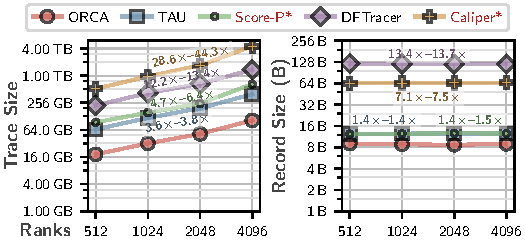
\includegraphics[width=\columnwidth]{amr_tracesizes_line.pdf}
    \caption{Trace size (left) and per-record size (right) comparison for detailed profile.
      ORCA traces are 3.6--44$\times$ smaller than other formats.
      Per-record size isolates format efficiency from record amplification --- other tracers emit
      2.5--3.3$\times$ more records than ORCA for the same collection profile.
    }
    \label{fig:orca:eval-tracesize}
  \end{figure}%
}

% Eval: Query suite only, one-column
\newcommand{\figEvalQueryOnly}{%
  \begin{figure}[t]
    \centering
    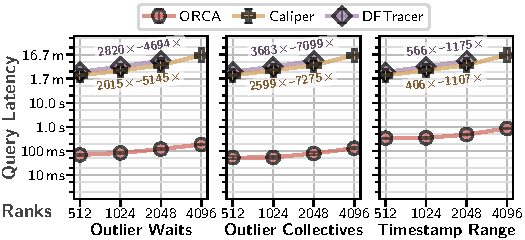
\includegraphics[width=\columnwidth]{query_suite_abs.pdf}
    \caption{Post-mortem query latencies on 20 timesteps.
      ORCA queries execute in O(100 ms), 3--4 orders of magnitude faster than
      \dftracer{} and Caliper.
      Performance for plaintext formats is dominated by parsing, not query complexity.
      TAU and \scorep{} are omitted as OTF2 is not a queryable format.
    }
    \label{fig:orca:eval-query}
  \end{figure}%
}

% Eval: Architecture comparison (OFI/TCP + DFTracer compression)
\newcommand{\figEvalArch}{%
  \begin{figure}[t]
    \centering
    \begin{subfigure}[t]{0.65\columnwidth}
      \centering
      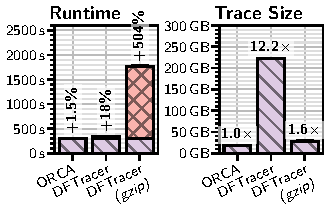
\includegraphics{dftracer_comp.pdf}
      \caption{Compression impact.}\label{fig:orca:eval-arch-dft}
    \end{subfigure}
    \hfill
    \begin{subfigure}[t]{0.33\columnwidth}
      \centering
      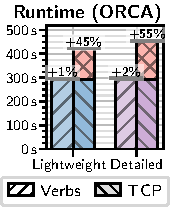
\includegraphics{ofi_tcp_tracer_runtimes.pdf}
      \caption{Transport impact.}\label{fig:orca:eval-arch-tcp}
    \end{subfigure}
    % \caption{Architectural analysis at 512 ranks. (Left) Enabling compression for \dftracer{}
    %   reduces trace size but increases runtime overhead due to CPU contention; ORCA's columnar
    %   format achieves comparable compression without this tradeoff. (Right) RDMA transport
    %   achieves lower overhead than TCP by bypassing the kernel.}
    \caption{(Left) Compression reduces trace size but induces severe jitter on simulation ranks.% --- \dftracer{} with gzip degrades to 504\% overhead.
      ORCA avoids this by offloading compression to dedicated aggregators.
      (Right) TCP transport increases ORCA overhead from 1--2\% to 45--55\%.
      Arrow-RDMA co-design is essential for low overhead.
    }
    \label{fig:orca:eval-arch}
  \end{figure}%
}

% Eval: Online vs offline
\newcommand{\figEvalOrcaNative}{%
  \begin{figure}[t]
    \centering
    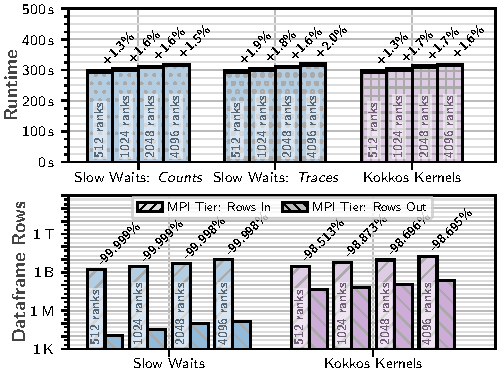
\includegraphics[width=\columnwidth]{ontv_combined.pdf}
    % \caption{In-situ analytics with operator pushdown.
    %   Runtime overhead remains below 2\% across all flows despite executing pushed-down operators on MPI
    %   nodes.
    %   Pushdown reduces transmitted data volume by 98.5--99.999\%, enabling continuous observability that
    %   would be impractical with capture-everything tracing.
    % }
    \caption{Runtime overhead (top) and MPI tier data reduction (bottom) for in-situ analytics with operator pushdown.
      Flows range from monitoring communication outliers to compute load balance.
      Pushdown discards 98.5--99.999\% of data at sub-2\% overhead, despite operators executing on MPI
      ranks.
    }
    \label{fig:orca:eval-ontv}
  \end{figure}%
}

% Eval: Verbs vs TCP
\newcommand{\figEvalOrcaTcp}{%
  \begin{figure}[t]
    \centering
    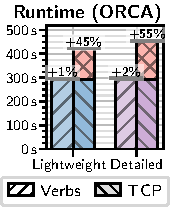
\includegraphics[width=\columnwidth]{ofi_tcp_tracer_runtimes.pdf}
    \caption{Transport comparison: RDMA verbs vs TCP.
      RDMA achieves lower and more consistent overhead by bypassing the kernel and avoiding jitter from
      socket operations.
    }
    \label{fig:orca:eval-tcp}
  \end{figure}%
}

% Eval: Agentic debugging timeline
\newcommand{\figEvalAgentic}{%
  \begin{figure}[t]
    \centering
    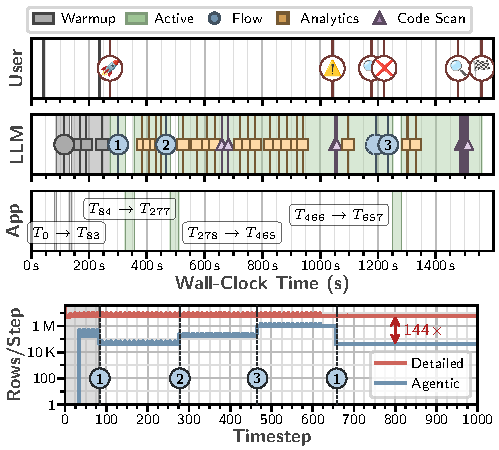
\includegraphics[width=\columnwidth]{agentic_timeline.pdf}
    % \caption{Agentic debugging session. (Top) User and LLM interactions over time, with numbered
    %   flow installations. (Bottom) Per-timestep event volume showing how the agent progressively
    %   narrows collection scope---from monitoring collectives to filtering Kokkos events to
    %   capturing targeted traces---localizing the anomaly from \Cref{fig:orca:bg-volatile} in minutes.}
    \caption{Visual transcript of an agentic debugging session demonstrating closed-loop capabilities.
      An LLM agent is tasked with localizing the anomaly from \Cref{fig:orca:bg-volatile} using high-level
      metrics, progressively collecting targeted telemetry to identify the source.
      The agent operates largely autonomously, producing the complete call path in 27 minutes.
      Reverting to baseline monitoring reduces data volume by 144$\times$.
    }
    \label{fig:orca:eval-agentic}
  \end{figure}%
}

% Eval: In-situ analytics flows table
\newcommand{\tablesink}[1]{\textcolor{gray!80}{$\rightarrow$ \emph{#1}}}
\newcommand{\tablevar}[1]{\texttt{\textit{\textcolor[HTML]{4D6B5A}{#1}}}}
\newcommand{\tabEvalFlows}{%
  \begin{table}[t]
    \centering
    \footnotesize
    \begin{tabular}
      {@{}p{2.3cm}p{5.6cm}@{}}
      \toprule
      \textbf{Flow}         & \textbf{Query}                                                            \\
      \midrule
      Outlier Wait~Counts   &
      \texttt{SELECT COUNT(*) FROM mpi\_wait WHERE~duration > 1ms} \tablesink{DuckDB}                   \\
      \addlinespace
      Outlier Wait~Traces   &
      \texttt{SELECT * FROM mpi\_wait WHERE~duration~>~1\,ms} \tablesink{Parquet}                       \\
      \addlinespace
      Load \mbox{Imbalance} &
      \texttt{SELECT rank, SUM(duration) FROM kokkos WHERE name IN \textcolor{gray}{<compute kernels>}} \\
                            & \texttt{GROUP BY rank} \tablesink{\tablevar{stats}} \tablesink{Parquet}   \\
      \addlinespace[0.2em]
                            & \texttt{PERCENTILES(\tablevar{stats}, 50/90/99\textsuperscript{th})} \tablesink{DuckDB}     \\
      \bottomrule
    \end{tabular}
    \caption{In-situ workflows evaluated in \S\ref{sec:orca:eval-insitu}, ranging from lightweight metrics and selective tracing on the communication path to aggregates over compute kernels.}\label{tab:ontv-flows}
  \end{table}%
}

\begin{document}
\renewcommand\linenumberfont{\normalfont\tiny\color{red}}
\linenumbers

% \title{ORCA: Real-time Observability and Control for Bulk-Synchronous~Parallel Applications}
\title{ORCA: Steerable Observability for Bulk-Synchronous~Parallel~Applications}

% -- ACM author --
% \author{CMU}

% -- IEEE author --
\author{\IEEEauthorblockN{Anonymous authors}}
% \IEEEauthorblockA{CMU}}

% -- IEEE: maketitle before abstract --
\maketitle

\begin{abstract}
  The \emph{bulk-synchronous parallel} (BSP) paradigm powers critical computational workloads from
  scientific simulations to large-scale machine learning training.
  Running on tens of thousands of processors, these systems are uniquely sensitive to performance
  variations that current observability approaches struggle to diagnose---post-hoc analysis of
  massive traces introduces latency and rigidity that obstructs timely diagnosis.

  To address these challenges, we present ORCA, a system for always-on, steerable BSP observability.
  ORCA enables operators to materialize relevant views from running applications on demand and
  intervene in response, via a tree-based overlay providing coordinated collection, in-situ SQL
  analytics, and timestep-consistent control.
  ORCA accelerates observability workflows across the spectrum.
  On a real AMR code at 4096 ranks, ORCA collects equivalent traces at \mytilde{2}\% overhead (vs
  56–81\% for tracing tools), enables up to 7275$\times$ faster queries, and 99.999\% in-situ data reduction.
  In an LLM-driven evaluation of steerability, a performance anomaly that took months to
  diagnose manually is localized in 27 minutes.
  % analyzes them orders of magnitude faster, and reduces in-situ data volume by up to 99.999\%.
  %.%  on a real AMR code at 4096 ranks, it% collects detailed traces at 1--2\% overhead versus 56--81\% for existing tracers, executes% post-mortem queries orders of magnitude faster, and reduces in-situ data volume by up to 99.999\%.

  % To address these challenges, we present ORCA, a system for always-on, steerable BSP observability. ORCA enables operators to materialize relevant views from running applications on demand and intervene in response, via a tree-based overlay providing coordinated collection, in-situ SQL analytics, and timestep-consistent control.
  % We present ORCA, a system for closed-loop BSP observability.
  % ORCA enables operators to declaratively specify views materialized on demand via a tree-based
  % overlay providing coordinated collection, in-situ SQL analytics, and timestep-consistent control.
  % On a real AMR code at 4096 ranks, ORCA collects detailed traces at 1--2\% overhead versus 56--81\%
  % for existing tracers, executes queries orders of magnitude faster, and reduces data volume by
  % multiple orders of magnitude through in-situ analytics.
  % In an agentic evaluation of the closed-loop workflow, a performance anomaly that took months to
  % diagnose manually is localized in 27 minutes.
\end{abstract}



% -- ACM-specific --
% \setcopyright{none}
% \settopmatter{printacmref=false}
% \renewcommand\footnotetextcopyrightpermission[1]{}
% \keywords{TODO}

% -- ACM: maketitle after abstract --
% \maketitle

% ! TeX root = ../main.tex

\section{Introduction}


The \emph{bulk-synchronous parallel} (BSP)~\cite{Valia1990:BSP} paradigm powers critical
computational workloads, from scientific simulations to large-scale machine learning training.
These systems are uniquely fragile: at the scale of tens of thousands of processors, lockstep
execution means a single straggler can block cluster-wide progress at every synchronization point.
As ML training pushes BSP toward 100K GPUs~\cite{Salpe2026:100K} and scientific workloads grow in
tandem~\cite{Das2023:LargeScale,Stock2024:LargeScale}, the cost of undiagnosed performance
pathologies has become economically untenable.
Yet the causes are diverse and highly
context-dependent~\cite{\citeGroupVarHpc,\citeGroupVarAmr,\citeGroupVarRdma,\citeGroupVarMisc,\citeGroupML}
---load imbalance, poor task overlap, hardware variability---varying across clusters, workloads, and
scales.
Metrics~\cite{:Prometheus,Schwa2021:LDMS} provide baseline visibility but rarely enough workload
structure to attribute causes.
Tracing~\cite{Shend2006:TAU,Knupf2012:Score-P,2025:PytorchKineto,Devar2024:DFTracer,Boehm2016:Caliper}
can capture the fine-grained patterns needed for diagnosis, but prevailing approaches---exhaustive
collection to disk followed by expensive \emph{extract-transform-load}
(ETL)~\cite{Yildi2023:IOMax,\citeJainAmr} ---cannot provide feedback at the speed problems demand.
In a prior study of placement in AMR codes~\cite{\citeJainAmr}, isolating the root causes of
several performance artifacts took months, while fixes typically took days.
Rapid visibility into production pathologies remains one of the highest-yield paths to efficiency.

We argue for always-on, steerable observability as a production capability for BSP workloads, not
just faster post-hoc analysis, but continuous visibility with the ability to escalate on demand.
The evolution of distributed tracing~\cite{Barha2004:Magpie,Fonse2007:X-Trace,Sigel2010:Dapper}
offers an instructive parallel.
In microservices, tracing evolved to preserve causal relationships between requests (the unit of
work in asynchronous systems) so tail latency is continuously monitored and attributable to
specific services.
In BSP, causality is induced by synchronization: performance anomalies manifest as stragglers that
stall collectives.
The same synchronization creates natural windows for both observation and intervention, enabling
operators to steer collection on demand, test hypotheses live, and act on feedback while the
job runs.
Real-time diagnostics are already proving valuable in ML training~\cite{\citeGroupML} for problems
ranging from straggler localization to training correctness, but each system implements a bespoke
collection and analytics pipeline.
% And because BSP is a single coordinated workload, the system can unify observation and% intervention---enabling operators to steer collection on demand, test hypotheses live, and act on% feedback, all while the job runs.
%A common observability substrate is needed for BSP workloads, 
BSP workloads need a common observability substrate, providing low-overhead on-fabric transport,
BSP-aware coordination semantics for telemetry aggregation and control, and programmable analytics
interfaces (\S\ref{sec:orca:req}).

We present a tree-based overlay~\cite{Arnol2006:TBONs} for rapid feedback loops over large-scale BSP
applications called 
ORCA~(\emph{Observability~with~Real-time~Control~and~Aggregation}).
ORCA treats telemetry as columnar streams and provides in-situ SQL-based
analytics, faster offline analytics, and a control plane for
online steerability.
Central to the design is treating synchronization as the fundamental consistency boundary.
On the data path, this yields \emph{timestep dataframes}~(\S\ref{sec:orca:des_model}): a
per-timestep grouping of all ranks' telemetry into a single logical analysis unit.
Because synchronization partitions BSP execution into causally independent windows, timestep
dataframes support both in-situ analysis during execution and timestep-partitioned persistence
for faster offline queries.
Combined with columnar formats (Arrow~\cite{:ApacheArrow} in transit, Parquet~\cite{:ApacheParquet} at rest), this eliminates the ETL
that dominates conventional tracing workflows.
An RDMA-based transport~(\S\ref{sec:orca:des_xport}) minimizes collection overhead,
while distributed query planning with operator pushdown minimizes data movement~(\S\ref{sec:orca:des_insitu}),
On the control path, a timestep-consistent commit protocol (\S\ref{sec:orca:des_ctl}) enables atomic
interventions---new analytics, probes, or parameter updates---applied asynchronously at the same timestep
across all ranks.
% Together, these enable workflows ranging from faster offline analytics to low-overhead, real-time, closed-loop feedback.
We evaluate ORCA on a real AMR code at 512--4096 CPU ranks:

% control paths to realize low-overhead, real-time, closed-loop feedback.
% We evaluate ORCA on a real AMR code at 512--4096 CPU ranks:

% We present a tree-based overlay for real-time observability and control of large-scale BSP applications called ORCA.
% ORCA treats telemetry as columnar streams and provides capabilities ranging from in-situ SQL-based analytics,
% faster dataframe-style offline analytics, and a control plane for online steerability.
% % ORCA provides timestep-consistent control and data
% ORCA constructs a tree-based overlay providing data and control paths
% both treating synchronization as the fundamental consistency boundary in BSP execution.
% On the data path, this yields an abstraction called timestep dataframe, consisting of all ranks' telemetry from a single timestep.
% As timesteps are causally independent, timestep dataframes enable in-situ analyses, and timestep-partitioned 
% layouts for faster offline analyses. Combined with columnar formats like Arrow and Parquet, this enables

% ORCA treats the synchronization window as the fundamental consistency boundary in BSP execution

% We present a \emph{tree-based overlay network} (TBON)~\cite{Arnol2006:TBONs} for real-time
% observability and control of large-scale BSP applications, called
% ORCA~(\emph{Observability~with~Real-time~Control~and~Aggregation}).
% ORCA treats telemetry as columnar streams, transformed in-situ via SQL-based analytics 
% %interface called \emph{OrcaFlow} 
% en route to \emph{sinks} such as dashboards or parallel filesystems.



% A key contribution is the timestep dataframe abstraction: recognizing that global synchronization
% divides BSP execution into causally independent windows, ORCA makes timestep the key thing
% for in-situ and offline  something.
% Timestep dataframes, consisting of all telemetry from a single timestep, enable both faster offline
% analysis by partitioning, and in-situ analysis too.
% Distributed query planning with operator pushdown minimizes data movement for in-situ analysis,
% (\S\ref{sec:orca:des_insitu}), while an end-to-end columnar pipeline enables zero-ETL post-mortems.

% A key contribution is the \emph{timestep dataframe} abstraction: building on the insight that
% global synchronization divides BSP telemetry into causally independent windows, ORCA transforms
% telemetry from a rank-major to a timestep-major representation (\S\ref{sec:orca:des_model}).
% An RDMA-based TBON-optimized transport (\S\ref{sec:orca:des_xport}) enables low-overhead collection of
% these dataframes.
% They can then be transformed via SQL-based analytics, routed to a dashboard, or persisted as
% partitioned Parquet for zero-ETL post-mortems.
% Distributed query planning with operator pushdown minimizes data movement across the overlay
% (\S\ref{sec:orca:des_insitu}).

% A control plane (\S\ref{sec:orca:des_ctl}) provides atomic and timestep-consistent control semantics,
% guaranteeing correctness for interventions such as new analytics, probes, parameter updates.
% ORCA combines a modern columnar analytics
% stack~\cite{:ApacheArrow,:ApacheParquet,Lamb2024:DataFusion} with RDMA and BSP-aligned data and
% control paths to realize low-overhead, real-time, closed-loop feedback.
% We evaluate ORCA on a real AMR code at 512--4096 CPU ranks:

\begin{itemize}[leftmargin=*]
  \item In conventional tracing workflows, ORCA captures equivalent telemetry at \mytilde{2}\% runtime overhead
        (vs 56--81\% for state-of-the-art tracers), produces up to 42$\times$ smaller traces, and
        enables up to 7275$\times$ faster offline analyses (\S\ref{sec:orca:eval-trace}).
  \item In-situ analytics enable low-overhead needle-in-the-haystack
        workflows---outlier \mpiw{} calls are isolated in real-time at sub-2\% runtime
        overhead, while discarding up to 99.999\% of data at MPI ranks (\S\ref{sec:orca:eval-insitu}).
  \item In an agentic evaluation of its steerable capabilities using an LLM
        agent,
        ORCA enables localizing a performance anomaly---the same bug from \cite{\citeJainAmr} that took
        months of manual investigation---in 27 minutes, while reducing data volume by up to 144$\times$
        (\S\ref{sec:orca:eval-agent}).
\end{itemize}

More broadly, ORCA demonstrates that declarative SQL analytics can be embedded on the fabric
alongside a live MPI application, enabling streaming analytics workflows beyond observability~(\S\ref{sec:orca:related}).
ORCA is open source~\cite{Autho2026:orca-code}.

% ! TeX root = ../main.tex

\section{Background and Motivation}\label{sec:orca:bg}

\emph{Bulk synchronous parallel} (BSP)~\cite{Valia1990:BSP} workloads in both scientific computing and machine learning
training pose unique efficiency challenges.
These jobs, increasingly spanning tens of thousands of nodes, execute in lockstep and synchronize
frequently via collective communication.
At these scales, BSP is uniquely fragile: a single straggler can block cluster-wide progress at
synchronization points.
Their root causes are highly context-dependent, ranging from load imbalance and suboptimal overlap
to tuning-induced variability, and have been documented
extensively~\cite{\citeGroupVarHpc,\citeGroupVarAmr,\citeGroupVarRdma,\citeGroupVarMisc,\citeGroupML}.
Despite extensive case studies, performance pathologies persist and remain costly to diagnose and
fix.

We argue this reflects a structural limitation in how BSP observability is practiced.
While monitoring infrastructure is widely deployed~\cite{:Prometheus,Schwa2021:LDMS}, it targets
\emph{known unknowns} via a fixed set of metrics such as CPU utilization.
Performance pathologies are dominated by \emph{unknown
  unknowns}~\cite{Major2017:o11y,:OtelO11y,Sridh:DistributedSystemsObservability} ---
they cannot be anticipated by predefined metrics, and resolving them requires iterative
investigation at varying resolutions: from high-level aggregates to fine-grained detail when
needed.
Current approaches to capturing fine-grained telemetry --- large event traces followed by
post-mortem analyses --- incur prohibitive collection and analysis
costs~\cite{Yildi2023:IOMax,\citeJainAmr}, delaying interventions.
As a result, operators are forced to choose between expensive investigations and ad-hoc
workarounds.
This gap motivates a different model: always-on application observability as a production
capability, with relevant views constructed on demand in real-time, hypotheses tested live, and
collection steered accordingly while the job is still running --- a paradigm we call
\emph{steerable observability}.

We now illustrate this gap with case studies from HPC and ML training (\S\ref{sec:orca:bg:studies}),
survey existing approaches and their limitations (\S\ref{sec:orca:bg:gaps}), and use our experiences
with eBPF~\cite{:eBPF} to motivate a programmable substrate for real-time visibility at workload
scale (\S\ref{sec:orca:bg:missing}).

% This gap motivates a different model: always-on observability as a production capability, with
% relevant views derived in real-time, hypotheses tested live, and collection steered accordingly
% while the job is still running --- a paradigm we call \emph{steerable observability}.
% Performance pathologies are dominated by \emph{unknown
%   unknowns}~\cite{Major2017:o11y,:OtelO11y,Sridh:DistributedSystemsObservability} ---
% resolving them requires constructing the right views from telemetry and refining them until causal
% attribution is possible.
% Dominant paradigms make this loop slow and rare: diagnosing pathologies requires rerunning
% applications under progressively heavier diagnostics, from lightweight profiles to fine-grained
% per-rank traces, followed by expensive \emph{extract-transform-load} (ETL)~\cite{Yildi2023:IOMax}
% before queries can be served.
% As a result, operators are forced to choose between expensive investigations and ad-hoc
% workarounds.
% This gap motivates a different model: always-on observability as an operational capability, with
% relevant views derived in real-time, hypotheses tested live, and collection steered accordingly
% while the job is still running.


\subsection{Case Studies from HPC and ML}\label{sec:orca:bg:studies}

\subsubsection{Optimizing Placement in AMR}
\figBgVolatile{}

% Our study of placement and load-balancing in \emph{adaptive mesh refinement} (AMR)
% codes~\cite{\citeJainAmr} illustrates this gap concretely.
A prior study of placement and load-balancing in \emph{adaptive mesh refinement} (AMR)
codes~\cite{\citeJainAmr} illustrates this gap concretely.
While widely known for load-imbalance challenges~\cite{Dubey2014:Survey}, the study finds
load-imbalance indistinguishable from other hardware, software, and tuning artifacts without
fine-grained telemetry.
\Cref{fig:orca:bg-volatile} shows one such example: tail latency spikes in \mpiw{}
that only manifested at scale would get attributed to collectives in aggregate telemetry.
Diagnosing each artifact required months of iterative investigation, while mitigations typically took days.

The primary diagnostic bottleneck was a slow feedback loop: each iteration required running the
codes, collecting large event traces, followed by post-mortem trace analyses bottlenecked on
expensive ETL (\emph{extract-transform-load}) from formats such as CSV.
Mitigations identified were cluster- and workload-specific.
Even after these artifacts were fixed, placement demonstrated a fundamental tradeoff
between compute load balance and communication locality --- the right balance between the two
varies across workloads, scales, and architectures.
Translating these optimizations to production environments would require repeating this
time-consuming exercise --- underscoring the need for infrastructure that makes such investigations
routine.
% Translating them to production environments would require repeating the same exercise.
% Given that optimal configurations are not portable across environments, the need is not for better
% one-off analyses but for infrastructure that makes such investigations routine.

\subsubsection{Parallels from the Pytorch Ecosystem}

The PyTorch~\cite{Paszk2019:PyTorch} ML training ecosystem exhibits the same offline feedback loop.
Kineto~\cite{2025:PytorchKineto} captures fine-grained traces on demand as JSON, triggered via a
node-local control daemon called Dynolog~\cite{2025:MetaDynolog}.
\emph{Holistic Trace Analysis} (HTA)~\cite{2025:MetaHTA} computes derived views such as activity
breakdowns and straggler detection.
Together, these cover capture, actuation, and analysis --- but HTA is a single-node
Pandas~\cite{:Pandas} script that cannot scale to cluster-wide traces, and Dynolog provides
best-effort actuation with no workload-level consistency guarantees.
% , whereas reliable construction of views like
% \Cref{fig:orca:bg-volatile} requires complete telemetry for each collective instance.

Recent ML training systems have begun addressing specific pathologies online --- straggler
localization~\cite{Yao2025:Holmes,Wu2025:GREYHOUND,\citeCuiXputimer,Guan2025:PerfTracker,Deng2025:Mycroft},
fault diagnosis~\cite{Dong2025:Aegis,Deng2025:Minder}, and training
correctness~\cite{Jiang2025:TrainCheck} --- but each reimplements subsets of collection,
aggregation, and control from scratch.
A common programmable substrate would generalize these diagnostics, allowing detection strategies
to be expressed as analytical queries over system state, composable without
rebuilding the underlying infrastructure.

\subsection{Existing Approaches and Gaps}\label{sec:orca:bg:gaps}

\parahead{Monitoring}
Monitoring enables basic cluster visibility via periodically captured metrics, but lacks the
workload context necessary to construct views like \Cref{fig:orca:bg-volatile}.
Widely deployed infrastructure for metrics includes Prometheus~\cite{:Prometheus}, a time-series
database, and LDMS~\cite{Schwa2021:LDMS}, an on-fabric hierarchical metric collection
infrastructure used in HPC clusters.

\parahead{Profiling and Tracing}
Tools such as TAU~\cite{Shend2006:TAU}, \scorep{}~\cite{Knupf2012:Score-P}, and
Kineto~\cite{2025:PytorchKineto} can provide both high-level aggregates via profiles or fine-grained telemetry
via traces, but are post hoc by design.
Traces can characterize short runs, but cannot provide always-on visibility over long-running jobs.
In the absence of any real-time feedback to guide collection, traces simultaneously overcollect
and undercollect --- despite capturing every \mpiw{}, they can not explain which sub-functions
within anomalous \mpiw{} caused the latency spikes.
Formats like OTF2~\cite{Eschw2012:OTF2} and JSON~\cite{:ChromeJsonTEF} 
require expensive transforms for dataframe-style analytics~\cite{Jain2025:AMR,Yildi2023:IOMax},
and visual inspection for anomalies is impractical for cluster-scale workloads.

% \cite{Bhate2019:Hatchet} (Hatchet)
% \cite{Yildi2023:IOMax} -- DFTracer cousin, exists because they do not know Polars + Lazy Parquet exists
\parahead{Dataframe Analytics}
Recent tools such as Caliper~\cite{Boehm2016:Caliper}, \dftracer{}~\cite{Devar2024:DFTracer},
Pipit~\cite{Bhate2024:Pipit}, and Pytorch HTA~\cite{2025:MetaHTA} have adopted
Pandas~\cite{:Pandas} and Dask-based~\cite{Rockl2015:Dask} dataframe analytics interfaces to
analyze telemetry, but require expensive ETL~\cite{Yildi2023:IOMax,\citeJainAmr} 
--- the working set for which scales with \emph{ranks $\times$ timesteps}.
%formats such as CSV and JSON 
Columnar formats like Parquet~\cite{:ApacheParquet} offer efficient post-hoc analytics, but do not
by themselves address overcollection, working set scaling, or real-time feedback, and remain
largely unadopted in tracing workflows.
In a simple internal port of HTA analyses from JSON to Parquet, we observed 12$\times$ faster data
loading and 8$\times$ faster end-to-end analysis.

% \cite{Godoy2020:ADIOS2} (ADIOS)
% \cite{Eisen2025:ADIOS} -- ADIOS SST
\parahead{Streaming and In-situ Analytics}
ADIOS~\cite{Godoy2020:ADIOS2} enables fixed-function in-situ workflows~\cite{Eisen2025:ADIOS} on
scientific data, typically run as another MPI application.
%provides transport abstractions for in-situ
MRNet~\cite{Roth2003:MRNet,Willi2016:MRNetApps} is a tree-based overlay used as a reduction backend
for commercial debuggers, but provides a compiled packet-based programming model.
Neither enable runtime-programmable dataframe-style analytics needed for real-time BSP
observability.
Cloud streaming systems such as Flink~\cite{Carbo2015:ApacheFlink} and Kafka~\cite{Kreps2011:Kafka}
are designed for independent event streams over IP networks They lack fabric-aware transport and
BSP-aligned coordinated collection, precluding views like \Cref{fig:orca:bg-volatile}.

\subsection{The Missing Substrate}\label{sec:orca:bg:missing}

Diagnosing the root cause behind \Cref{fig:orca:bg-volatile} required capabilities beyond what any
single tool in the taxonomy provides.
At node scale, eBPF~\cite{:eBPF} provides a template: dynamic probes, programmatic aggregation, low
overhead in the common case with depth when needed.
It enabled controlled and targeted access to telemetry within \mpiw{} after alternatives were
exhausted.
Hypotheses about interrupts and scheduler effects were tested and discarded in hours.
But eBPF is node-local, and our workflow involved ad-hoc orchestration, uncoordinated collection,
and manual post-hoc correlation.
Extending this to workload scale requires a substrate for real-time \emph{feedback}, treating
observability not as distributed logging, but as materializing views directly from running
applications.
But visibility alone is insufficient for steerability. Interventions --- whether additional views
or parameter adjustments --- require a \emph{control plane} back to the running application,
and may be driven by humans, automated agents, or policies.
The next section states the requirements such a substrate must satisfy.

\input{tex/03-chal}
\input{tex/04-design}
\input{tex/05-impl}
\input{tex/06-eval}
\input{tex/07-related}
\input{tex/08-concl}
% \section{References}
% \clearpage
\renewcommand*{\bibfont}{\small}
\printbibliography{}

% % ! TEX root = ../main.tex

\newlength{\tabOrcaYwidth}
\setlength{\tabOrcaYwidth}{\dimexpr(\textwidth - 1.0in - 1.5in - 8\tabcolsep) / 2\relax}

\newcommand{\tabOrcaRelatedInner}[1]{%
  \begin{tabular}
    [t]{@{}>{\raggedright\arraybackslash}p{1.5in}>{\raggedright\arraybackslash}p{\tabOrcaYwidth}>{\raggedright\arraybackslash}p{\tabOrcaYwidth}@{}}
    #1
  \end{tabular}%
}

\newcommand{\tabOrcaGreyhound}{%
  \tabOrcaRelatedInner{
    \textbullet~Iteration boundary detection & \textbullet~Autocorrelation over collectives & \textbullet~\texttt{PostTimestepAdvance} \\
    \textbullet~Fail-slow detection & \textbullet~Track iteration times & \textbullet~Track iteration times \\
    \textbullet~Straggler localization & \textbullet~Aggregate NCCL events (off-fabric) & \textbullet~\texttt{GROUPBY swid} (on-fabric) \\
    \textbullet~Straggler cause disambiguation & \textbullet~Microbenchmarks & \textbullet~Microbenchmarks or trace events \\
    \textbullet~Online interventions & \textbullet~Tune micro-batch distribution or parallelism & \textbullet~Supported via control plane \\
  }%
}

\newcommand{\tabOrcaFlare}{%
  \tabOrcaRelatedInner{
    \textbullet~Stall detection/disambiguation & \textbullet~Call stack analysis & \textbullet~In-situ reductions \\
    \textbullet~Slowdown analysis & \textbullet~Periodic metrics & \textbullet~In-situ trace event aggregation \\
  }%
}

\newcommand{\tabOrcaAegis}{%
  \tabOrcaRelatedInner{
    \textbullet~Fail-stop hardware & \textbullet~Per-node NCCL counters pulled on timeouts & \textbullet~Workload-level trace events \\
  }%
}

\newcommand{\tabOrcaHolmes}{%
  \tabOrcaRelatedInner{
    \textbullet~Outlier collective detection & \textbullet~Random forest model & \textbullet~Policy-dependent \\
    \textbullet~Localization & \textbullet~Graph search & \textbullet~Learn collective topology at bootstrap, \texttt{GROUPBY~swid}, trace critical path in reverse \\
  }%
}

\newcommand{\tabOrcaMycroft}{%
  \tabOrcaRelatedInner{
    \textbullet~Straggler detection/localization & \textbullet~Fine-grained trace NCCL events buffered locally, flushed to Kafka if heuristics trigger & \textbullet~Aligned dataframes analyzed in-situ \\
  }%
}

\newcommand{\tabOrcaTrainCheck}{%
  \tabOrcaRelatedInner{
    \textbullet~Correctness invariants & \textbullet~Offline trace analysis for invariant generation, online enforcement & \textbullet~Timestep-aligned traces for offline generation, in-situ enforcement via OrcaFlow \\
  }%
}

\newcommand{\tabOrcaReveal}{%
  \tabOrcaRelatedInner{
    \textbullet~Anomaly detection and attribution & \textbullet~Time-windowed metrics + unsupervised learning & \textbullet~Workload-level trace events \\
  }%
}

\newcommand{\tabOrcaMinder}{%
  \tabOrcaRelatedInner{
    \textbullet~Fail-slow hardware & \textbullet~Cluster-level metrics and anomaly detection & \textbullet~Workload-level trace events \\
  }%
}

\newcommand{\tabOrcaPerfTracker}{%
  \tabOrcaRelatedInner{
    \textbullet~Anomaly detection and attribution & \textbullet~Always-on iteration monitoring & \textbullet~Identical workflow, but workload-level \\
    & \textbullet~Trigger-driven detailed capture & \\
    & \textbullet~In-situ telemetry reductions & \\
  }%
}

\appendices
\section{ML Training Observability Comparison}\label{sec:appdx}

\newcommand{\tabOrcaRelated}{%
\begin{table*}[t]
  \hyphenpenalty=10000
  \exhyphenpenalty=10000
  \centering
  \scriptsize
  \newcolumntype{Y}{>{\raggedright\arraybackslash}X}
  \begin{tabularx}{\textwidth}{>{\raggedright\arraybackslash}p{1.0in} X}
    \toprule
    \textbf{System}                                                     &
    \tabOrcaRelatedInner{
    \textbf{Diagnostic Task}                                            & \textbf{Their Approach} & \textbf{ORCA Equivalent} \\
    }
    \\
    \midrule
    Greyhound~\cite{Wu2025:GREYHOUND} \emph{(Fail-slows)}               &
    \tabOrcaGreyhound                                                                                                        \\
    \midrule
    Flare~\cite{Cui2026:Flare} \emph{(Training~anomalies)}              &
    \tabOrcaFlare                                                                                                            \\
    \midrule
    Holmes~\cite{Yao2025:Holmes}\newline \emph{(Fail-slows)}                    &
    \tabOrcaHolmes                                                                                                           \\
    \midrule
    Mycroft~\cite{Deng2025:Mycroft} \emph{(Training~anomalies)}         &
    \tabOrcaMycroft                                                                                                          \\
    \midrule
    TrainCheck~\cite{Jiang2025:TrainCheck} \emph{(Training~correctness)} &
    \tabOrcaTrainCheck                                                                                                       \\
    \midrule
    Reveal~\cite{Chen2025:Reveal} \emph{(Training~anomalies)}           &
    \tabOrcaReveal                                                                                                           \\
    \midrule
    Minder\textsuperscript{\#}~\cite{Deng2025:Minder} \emph{(Fault~diagnosis)} &
    \tabOrcaMinder                                                                                                           \\
    \midrule
    Aegis\textsuperscript{\#}~\cite{Dong2025:Aegis} \emph{(Fault~diagnosis)}                &
    \tabOrcaAegis                                                                                                            \\
    \midrule
    PerfTracker\textsuperscript{\#}~\cite{Guan2025:PerfTracker} \emph{(Training~anomalies)} &
    \tabOrcaPerfTracker                                                                                                      \\
    \bottomrule
  \end{tabularx}
  {\par\vskip 0.2em\raggedright\scriptsize\itshape \textsuperscript{\#} Minder, Aegis, and PerfTracker target multi-tenant environments. ORCA currently supports a single large workload.\par}
  \caption{Diagnostic approaches in ML training observability and their ORCA equivalents.}\label{tab:orca:related-work}
\end{table*}%
}

\tabOrcaRelated{}

Recent ML training systems build application-specific pipelines spanning
straggler localization~\cite{Wu2025:GREYHOUND,Yao2025:Holmes,Deng2025:Mycroft},
fault diagnosis~\cite{Deng2025:Minder,Dong2025:Aegis}, and correctness
enforcement~\cite{Jiang2025:TrainCheck}.
ORCA generalizes the pattern.
Holmes~\cite{Yao2025:Holmes} uses graph search over collective telemetry to
find anomalies.
ORCA's aligned collection makes stragglers surface through
simple grouped aggregations, no complex detection needed.
Mycroft~\cite{Deng2025:Mycroft} buffers fine-grained NCCL~\cite{:NCCL} telemetry locally
and flushes to Kafka~\cite{Kreps2011:Kafka} on trigger, but notes the scalability limits of central
logging.
ORCA's tree-based overlay scales out naturally.
TrainCheck~\cite{Jiang2025:TrainCheck} enforces training correctness via
offline invariant generation and online checks.
ORCA's timestep-aligned columnar analytics accelerate both stages.
Minder~\cite{Deng2025:Minder},
Aegis~\cite{Dong2025:Aegis}, and PerfTracker~\cite{Guan2025:PerfTracker} operate at the cluster
infrastructure level,
using hardware counters, metrics, and fine-grained trace events to identify faulty nodes across
workloads.
Their scopes range from identifying bad hardware across many workloads treated as black boxes to
providing tuning recommendations to customers.
ORCA provides
high-fidelity visibility into a single workload but does not yet support
cross-workload diagnosis in multi-tenant environments.
\Cref{tab:orca:related-work} summarizes the diagnostic mechanisms implemented in these systems and
their ORCA equivalents.

Among these systems, Greyhound~\cite{Wu2025:GREYHOUND} and PerfTracker~\cite{Guan2025:PerfTracker}
are the closest to ORCA in scope.
Greyhound implements a complete feedback loop: iteration times are
tracked, NCCL events are collected for localization when outliers are
detected, microbenchmarks are dispatched to validate stragglers, and online
tuning rebalances work in response.
This is a fixed-function version of what ORCA expresses as composable operators.
ORCA's timestep dataframe abstraction preserves fine-grained trace events,
enabling disambiguation of stragglers without needing microbenchmarks for validation.
Greyhound's control semantics require pausing the application,
while ORCA implements an asynchronous control plane with atomicity and timestep-consistency
guarantees.
Additionally, ORCA's on-fabric broadcast tree enables faster message dissemination than a central
controller.
PerfTracker implements a two-level loop: lightweight always-on monitoring of iteration times, with
detailed capture triggered by outliers.
Node-level aggregation reduces 300\,MB of telemetry to 30\,KB of aggregated signatures.
Long symbol names are noted as contributing to size amplification, which ORCA avoids via
dictionary-encoded Arrow columns.
\end{document}
